\section{Structures} \label{section:structures}
\subsection{First Stage}

\begin{figure}
    \centering
    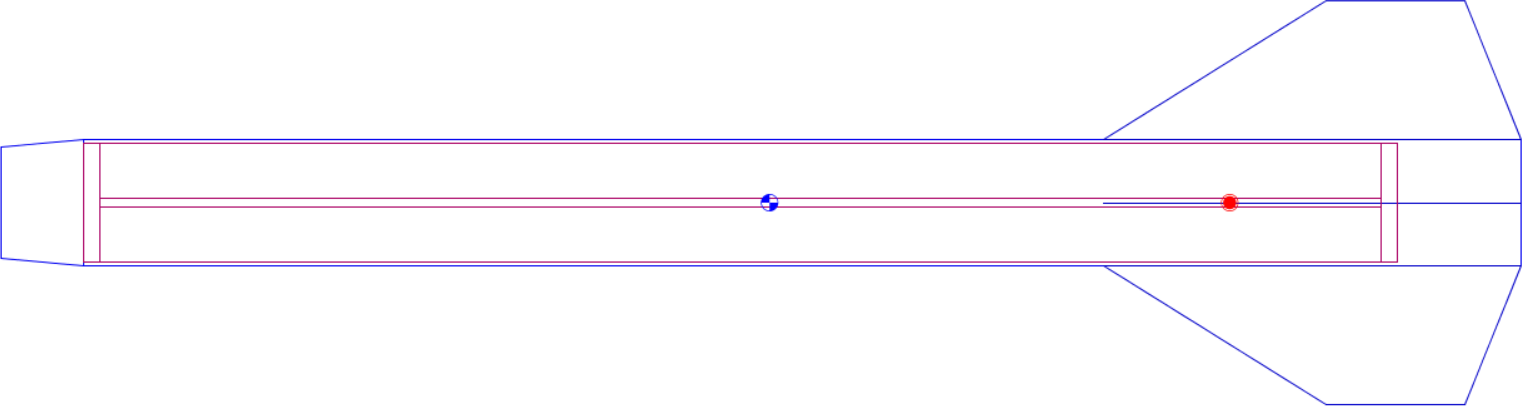
\includegraphics[width=0.8\textwidth]{images/expendable-booster}
    \\ \vspace{0.5cm}
    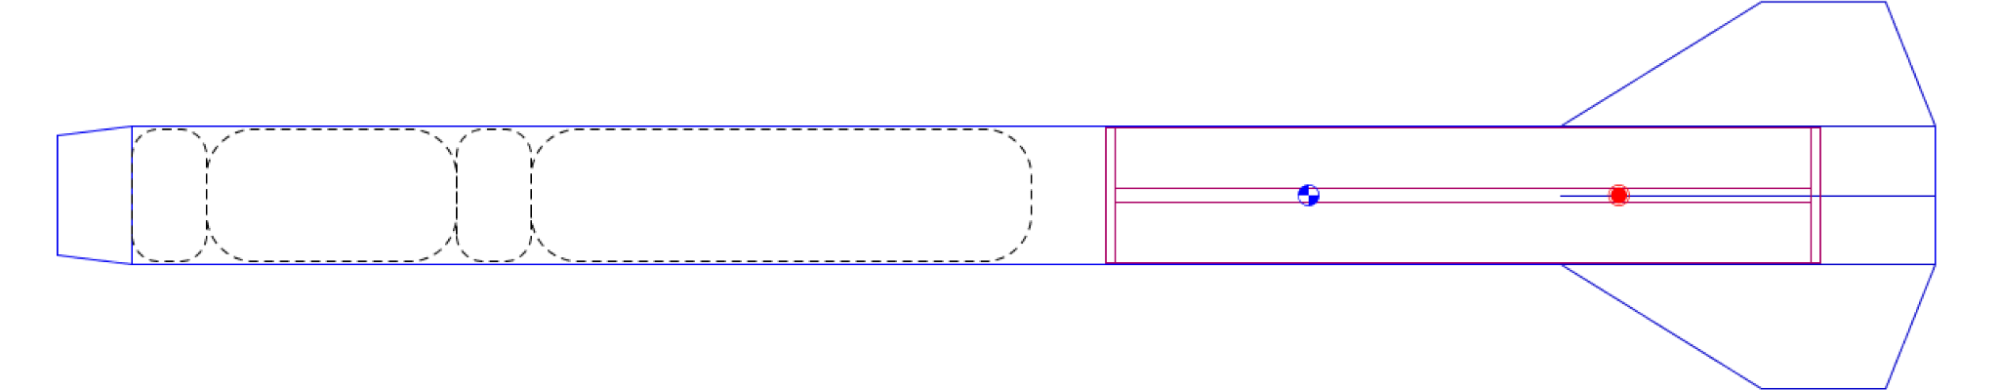
\includegraphics[width=0.8\textwidth]{images/recoverable-booster}
    \caption{Basic models of the 4.5'' expendable first stage (top) and the 5.5'' recoverable booster (bottom)}
    \label{figure:ork-boosters}
\end{figure}

The first stage must be able to withstand the structural and thermal loading that it will experience during the flight (\hyperlink{STR.2.2.1}{STR.2.2.1}, \hyperlink{STR.2.2.2}{STR.2.2.2}). As discussed previously, it is yet undetermined if the first stage may be expended. An expendable first stage will not need an avionics or recovery system, which would significantly reduce the weight of the stage and the design complexity. However, a recoverable booster stage is still under consideration and included in this review.


\subsubsection{First Stage Airframe}
Based on the sizing results, the optimal diameters for the first stage airframe are between 4.5'' and 5.5''. For the recoverable 5.5'' airframe, aluminum and titanium were considered and studied by our team. Since the recoverable first stage option slightly exceeds the mass budget estimated by the structure's sizing script, titanium as a material for the first stage was eliminated. In addition, the heating effects on the booster stage are not as significant as the sustainer stage, making aluminum a valid decision for the first stage. That airframe diameter makes buying or machining the tube feasible. A 1/4'' thick aluminum 6061 tube is available that satisfies safety factor requirements (\hyperlink{STR.2.3}{STR.2.3}).

For the 4.5'' expendable option, aluminum is still the leading option for the airframe material. Since all point designs are sub-minimum diameter, the airframe will act as the motor casing. Aluminum is the best material that can withstand the internal pressure and the heating effects expected on the first stage during flight. A 1/8'' wall thickness Aluminum 6061 tube is available that satisfies safety factor requirements.


\subsubsection{First Stage Fins} \label{section:s1-fins}

For preliminary sizing of lower fins, off-the-rail stability margin, fin flutter velocity and ease of manufacturability were evaluated. Fin flutter is a serious design concern at supersonic speeds, as when speeds increase, the likelihood of the fins vibrating at their resonance frequency and breaking increases as well.

\begin{figure}
    \centering
    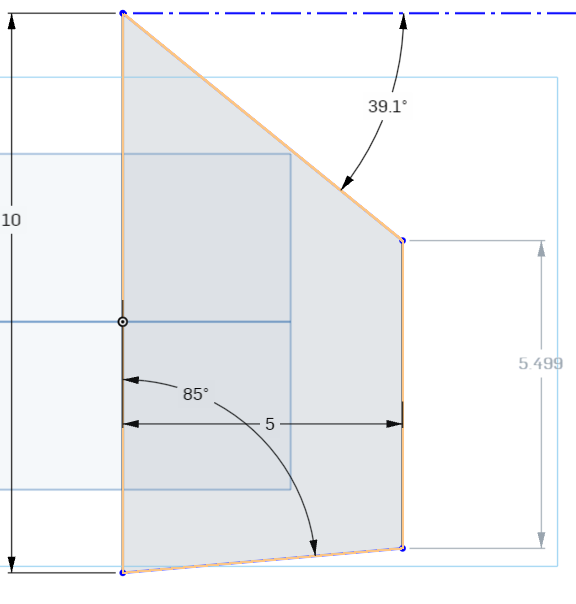
\includegraphics[width=0.6\textwidth]{images/lower-fin-design}
    \caption{``Combo Bonus'' fin geometry}
    \label{figure:combo-bonus}
\end{figure}

Three fin options were created based on research of prior art. The current leading candidate fin geometry, dubbed ``Combo Bonus'', consists of a geometry as depicted in \Cref{figure:combo-bonus}, with a thickness of 2 mm of titanium (\hyperlink{STR.1.4}{STR.1.4}). The projected number of fins is 4, in order to manage the center of pressure while minimizing the necessary size of fins, as larger fins are more susceptible to fin flutter (\hyperlink{STR.1.3}{STR.1.3}). 

The thickness of the fins was chosen to be 2 mm to reduce the chance of fin flutter while keeping the fins relatively light. 2 mm thick fins allow for fin flutter stability with the thinnest fins possible, based on the analysis below. The tip chord was chosen to determine the size of the fins (\hyperlink{STR.1.7}{STR.1.7}). The leading edge is the most important factor, as a 39.1 degree leading edge maximizes the safe velocity without fin flutter \cite{lf2} (\hyperlink{STR.1.10}{STR.1.10}). The edge opposite to the leading edge was chosen at 85 degrees, to increase stability by reducing the length of the root chord slightly. 

Fin flutter velocity as a function of altitude was calculated to evaluate the feasibility of the ``Combo Bonus'' design, using \Cref{equation:fin-flutter}. An Openrocket file of the 4.75'' - 4'' expendable rocket point design was used to vary the fin geometry and evaluate the off-the-rail stability margin. A stability caliber of above 1.5 is generally recommended for high power rockets.

\begin{figure*}
    \begin{equation} \label{equation:fin-flutter}
        V = \frac{a}{\sqrt{P}} \sqrt{\frac{G}{\left[\frac{1.337 (AR)^3 (l + 1)}{2 (AR + 2) \left(t/c\right)^3}\right]}}
    \end{equation}
    \caption*{Fin flutter velocity equation (from \cite{lf1})}
\end{figure*}

Many different considerations were made regarding fin attachment methods. It is important to select a method that can withstand the high structural and thermal loads the rocket will be subjected to (\hyperlink{STR.4.2.1}{STR.4.2.1}, \hyperlink{STR.4.2.2}{STR.4.2.2}). An additional complication comes from the sub-minimum diameter airframe: no through-the-wall methods near the pressure vessel are feasible, and welding was deemed too risky. The main methods of attachment considered were a customized fin can, a fin bracket attached to the nozzle walls, and a leading edge hoop attachment with lower edge bracket. The customized fin can was well demonstrated by the Princeton SpaceShot vehicle \cite{princeton}. The quarters of the fin can are manufactured individually and then a high temperature epoxy is applied to join the quarters together to create a cohesive fin can, shown in \Cref{figure:princeton-fin-can}. This method provides liberty in choosing materials as well as high structural integrity, however it requires a long manufacturing process.

\begin{figure}
    \centering
    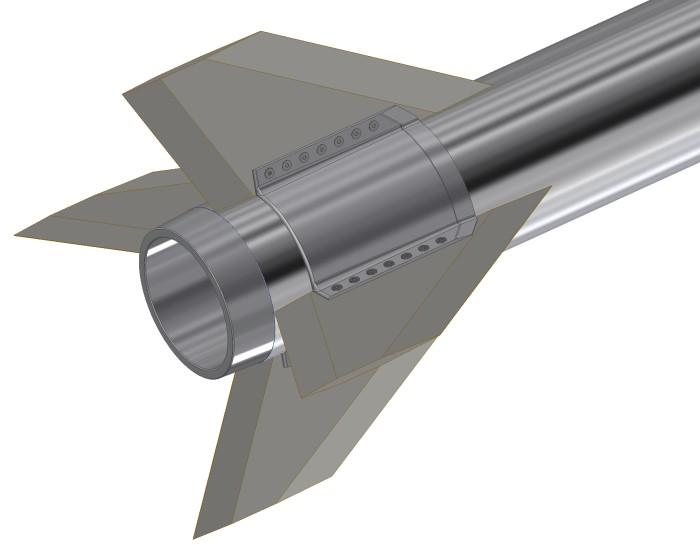
\includegraphics[width=0.6\textwidth]{images/princeton-fin-can}
    \caption{Princeton SpaceShot fin can CAD (from \cite{princeton})}
    \label{figure:princeton-fin-can}
\end{figure}

While it is impossible to drill into the airframe where the motor pressure vessel is, the airframe furthest aft, near the nozzle, is not a pressure vessel. The fin bracket method takes advantage of this by drilling into the nozzle casing to create brackets bolted into the nozzle casing that line the rocket body up to the leading edge of the fins. The fins are then attached to this bracket on the edge closest to the rocket body. 

Another option is to have a leading edge hoop with a lower edge bracket, aimed to make the fins more stable with only a small amount of additional manufacturing. The idea behind this design is to take advantage of the 5 inch nozzle throat section to secure the fins to the body similarly to the fin bracket method. Then, to ensure the fins remain stable even at the leading edges, the band will secure the other end around the combustion chamber.

The pictures below show examples of possible fin attachment methods. In \Cref{figure:bolts-and-brackets}, bolts are used to attach the fin trailing edge to the bottom of the motor casing and brackets to attach the fin root chord. From \Cref{figure:fin-diagram}, the second method is preferable -- two brackets bolted to the bottom of the motor casing (with the fin between the brackets). The optimal method for mounting and bolt configuration will be determined in the future through analytical structural analysis and FEA.

The fin attachment methods discussed in this section are equally applicable to the fins on both stages, since both stages are sub-minimum diameter.

\begin{figure}
    \centering
    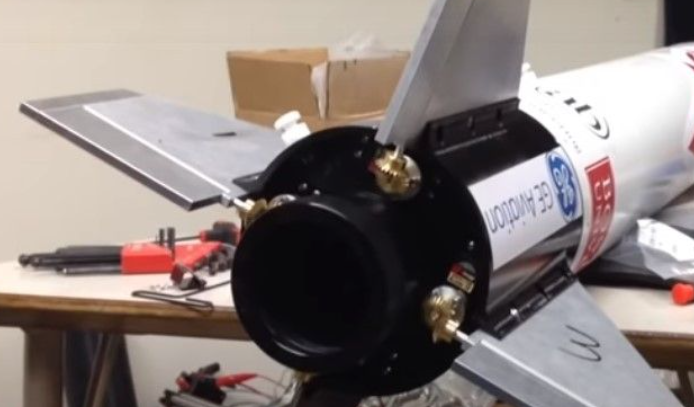
\includegraphics[width=0.6\textwidth]{images/fin-example}
    \caption{Fins attached using bolts and brackets (from \cite{bu-astro})}
    \label{figure:bolts-and-brackets}
\end{figure}

\begin{figure}
    \centering
    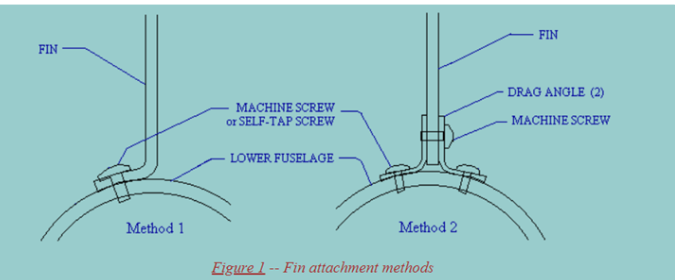
\includegraphics[width=0.7\textwidth]{images/fin-attach-diagram}
    \caption{Fin bolted at the bottom of motor casing (from \cite{nakka})}
    \label{figure:fin-diagram}
\end{figure}


\subsubsection{Interstage}
The current interstage design is currently unrefined, as this design review is being held early in the design process. For the sake of sizing, it was assumed to be a conical section three inches tall (\hyperlink{STR.3.3}{STR.3.3}). The wall thickness and material was kept constant with the first stage airframe (\hyperlink{STR.3.4}{STR.3.4}). Buckling and compressive safety factors were not calculated for this review as they can be assumed to be higher than the first stage airframe, as the structure is a short truncated cone with lower inertial loads than the first stage (\hyperlink{STR.3.2.1}{STR.3.2.1}, \hyperlink{STR.3.2.2}{STR.3.2.2}).


\subsection{Second Stage}
\begin{figure}
    \centering
    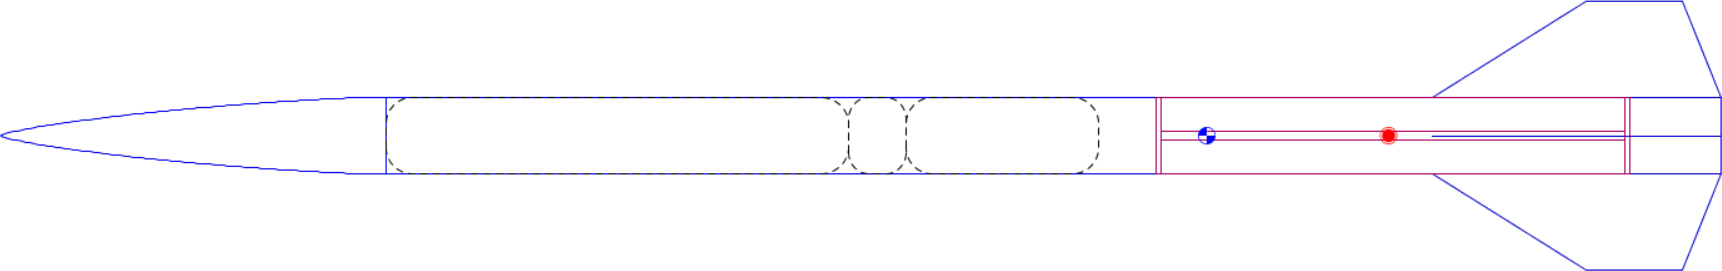
\includegraphics[width=0.8\textwidth]{images/small-sustainer}
    \\ \vspace{0.5cm}
    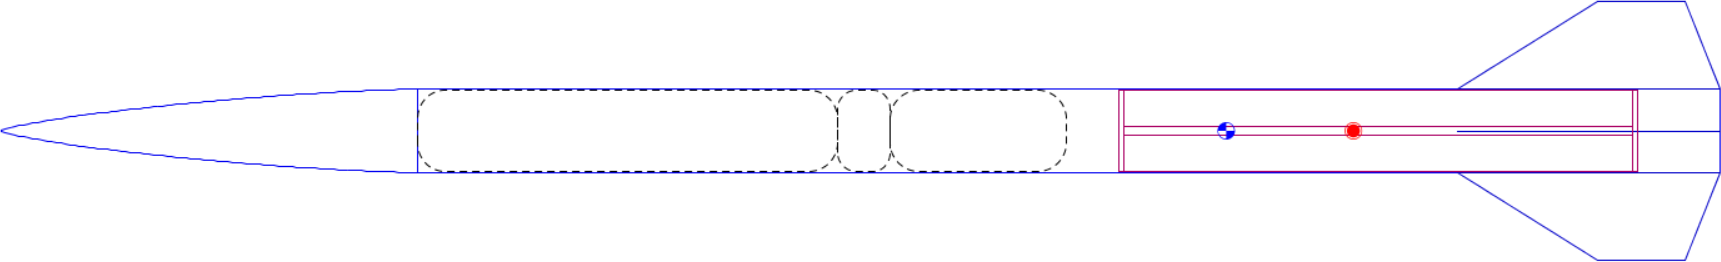
\includegraphics[width=0.8\textwidth]{images/large-sustainer}
    \caption{Basic models of the 4'' (top) and 4.75'' (bottom) second stage designs}
    \label{figure:ork-sustainers}
\end{figure}


\subsubsection{Second Stage Airframe}
The point designs for the second stage airframe have diameters from 4'' to 4.75'' with a thickness of 0.05'' (\hyperlink{STR.5.1}{STR.5.1}, \hyperlink{STR.5.3}{STR.5.3}). Those diameters have been selected through the sizing process, and the thicknesses were selected based on the available titanium tube sizes. Even with the 0.05'' thick tubes, the titanium airframes passed our first-order buckling and hoop stress analysis with safety factors over 3 (\hyperlink{STR.5.2.2}{STR.5.2.2}). Additionally, titanium was shown to be able to withstand the highest thermal loads of the materials considered (\hyperlink{STR.5.2.1}{STR.5.2.1}), and was shown to be effective at high Mach numbers in prior art. Titanium was selected for the sustainer since it maintains most of its strength for temperatures of over 800K, unlike aluminum \cite{jsr}.

\begin{figure}
    \centering
    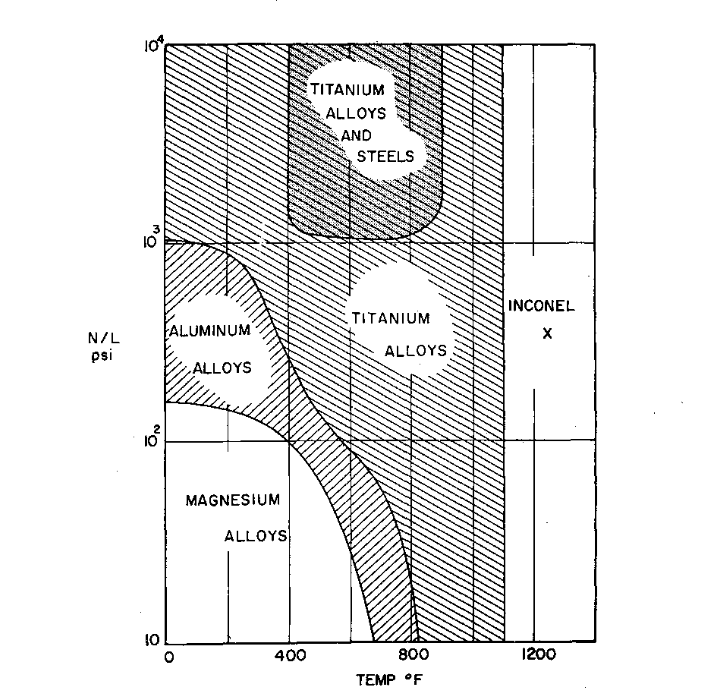
\includegraphics[width=0.5\textwidth]{images/temp-diagram}
    \caption{Material efficiency chart for stiffened cylinders in compression \cite{jsr}}
    \label{figure:temp-diagram}
\end{figure}


\subsubsection{Avionics Bay}
A section of the airframe on the second stage must be designed to accomodate the avionics system, which requires RF transparency so downlink can occur (\hyperlink{AVI.4}{AVI.4}). This requirement rules out materials like metals or carbon fiber for this section. The material selected for this section is fiberglass reinforced plastic. Based on our team's current, limited knowledge of electromagnetic wave propagation analysis, the height of the transparent section was set at 14 inches. Whether this is sufficient or excessive will be determined through future research and testing.

The main issue with a fiberglass avionics bay, as shown by the high altitude rocket created by University of Canterbury, is heat (\hyperlink{AVI.5.3}{AVI.5.3}). They mitigated the heat transfer to their RF transparent fiberglass section using a phenolic ablative resin that was externally applied to the tube \cite{into-black}. The phenolic is also RF transparent, and does not interfere with RF transparency.

In addition to RF transparency, the avionics system requires sampling holes, which allow the pressure inside the vehicle to equalize with the continuously changing ambient pressure, so the barometer can sample the pressure accurately (\hyperlink{AVI.1.1}{AVI.1.1}). The quantity and size of the sampling holes mainly depends on the diameter of the avionics bay. Thermal concerns caused by the sampling holes are still being researched. There may need to be some structure inside the vehicle that the incoming air must pass through before interacting with the avionics boards, to protect them. 


\subsubsection{Second Stage Fins}
Taking into account fin flutter and a stability caliber of about 2.6, the following preliminary geometry for the second stage fins is as follows:

\begin{itemize}
    \item Root Chord: 15'' (\hyperlink{STR.4.6}{STR.4.6})
    \item Tip Chord: 4'' (\hyperlink{STR.4.7}{STR.4.7})
    \item Height/Semi Span: 4'' (\hyperlink{STR.4.8}{STR.4.8})
    \item Sweep Length: 8.66'' (\hyperlink{STR.4.9}{STR.4.9})
    \item Sweep angle: 65.2\(^\circ\) (\hyperlink{STR.4.10}{STR.4.10})
\end{itemize}

The fin flutter velocity can be determined using the same methods as in \Cref{section:s1-fins}. The Mach number corresponding to the flutter velocity ranges from Mach 4.01 to 5.64 for an altitude range of 10K - 30K feet, and from 40K - 80K feet, the flutter velocity ranges from Mach 6.96 to 18.18. Currently, the rocket is predicted to reach high supersonic speeds (Mach 4); therefore flutter is only a concern untill an altitude of about 40 - 50K feet and not higher, once flutter velocity is significantly greater than rocket's velocity. Ideally, a factor of safety of 2 is needed for the fins. If the flutter Mach number doesn't meet this requirement throughout the rocket's velocity profile, the fin geometry parameters will need to be changed.  This would include reducing the aspect ratio, and increasing fin thickness (\hyperlink{STR.4.4}{STR.4.4}), which is currently estimated to be \(\sim\)0.1 inches \cite{lf1}.

It should be noted that the upper fin geometry is dependent on lower fin geometry (in terms of center of pressure and resulting stability margin off-the-rail), among other considerations such as thermal and structural loads (\hyperlink{STR.4.2.1}{STR.4.2.1}, \hyperlink{STR.4.2.2}{STR.4.2.2}). Currently, titanium is being considered for the upper fins due to its low thermal conductivity and because the sustainer stage is likely going to be made of titanium.

\begin{figure}
    \centering
    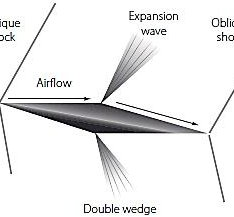
\includegraphics[height=3cm]{images/double-wedge} \hspace{1.5cm} 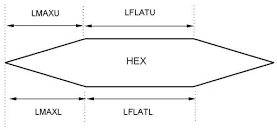
\includegraphics[height=3cm]{images/hexagonal}
    \caption{Double wedge airfoil cross section and hexagonal airfoil cross section}
    \label{figure:airfoil-cross-sections}
\end{figure}


\begin{table}
    \centering
    \begin{tabular}{cc||cc}
        \textbf{Metric} & \textbf{Weight} & Double Wedge & Hexagonal \\ \hline
        Cost & 7.5 & 7 & 7 \\ 
        Manufacturability & 10 & 1 & 10 \\ 
        Ease of Design & 5 & 2 & 7 \\ 
        Success Rate & 15 & 8 & 9 \\ 
        Performance & 12.5 & 9 & 8 \\ \hline 
         & \textbf{Totals:} & 305 & 422.5
    \end{tabular}
    \caption{Decision matrix for the fin cross-section geometry}
    \label{table:fin-cross-section-design-matrix}
\end{table}

The hexagonal design is by far the most realistic and feasible cross-sectional geometry for the second stage fins. Both cross-sections included in the matrix have hypothetically similar costs, assuming the same materials are used (a conventional airfoil was not considered due to extremely poor performance and high failure rate at supersonic speeds [2]).  The double wedge has superior flight performance and there are examples of it being used in real-world applications (see Figure 2).  However, after discussing with the manufacturing lead, it was determined that the double wedge would be next to impossible to manufacture compared to the hexagonal design. Combine this with only small marginal differences in the drag characteristics of the two cross-sectional geometries, as well as the fact that the hexagonal shape provides slightly better stability in flight, the hexagonal cross-section is easily the best choice for the upper fins.


\subsubsection{Nosecone}

For the preliminary sizing of the nosecone, several different geometries and their individual performances across several Mach numbers were evaluated. The nosecone should cause the least amount of drag possible (\hyperlink{STR.6.7}{STR.6.7}) and should also be able to survive the expected thermal (\hyperlink{STR.6.2.1}{STR.6.2.1}, \hyperlink{STR.6.3.1}{STR.6.3.1}) and structural loads (\hyperlink{STR.6.2.2}{STR.6.2.2}, \hyperlink{STR.6.3.2}{STR.6.3.2}) at all speeds. Based on this research, it was determined that although power series nosecones have the lowest drag coefficients above the transonic region, the Von K\'{a}rm\'{a}n profile with a fineness ratio of 5:1 had superior performance in the transonic region and thus may be the best choice (\hyperlink{STR.6.1}{STR.6.1}).

The expected steady state temperature at the nosecone tip will be around 1350K, based on flight at Mach 5.7 at 40,000 ft \cite{fleeman}. To account for such temperatures, the nosecone must be made out of titanium to maintain its high strength. Aluminum, for example, would lose 90\% of its strength if it were exposed to these temperatures. At flight to around Mach 4.5, titanium and its alloys would be the preferred material to survive the thermal and structural loads, while at speeds up to Mach 5.7, alloys such as Inconel must be used to survive \cite{fleeman}. The tip of the nosecone will either remain as titanium or be made out of Inconel. That decision will be driven futher flight modelling and a more accurate maximum Mach number.

The manufacturability of the nosecone material is extremely important to consider given the need for machining. Titanium, while extremely durable and heat resistant, is also expensive and difficult to machine with traditional subtractive manufacturing techniques. Inconel is similar, with high strength and temperature resistance making it extremely difficult to machine.

\begin{figure}
    \centering
    \begin{tikzpicture}
        \begin{axis}[
            width=14cm,
            height=8cm,
            xlabel={Mach Number},
            ylabel={Drag Coefficient},
            xmin=0.0, xmax=8.0,
            ymin=0.0, ymax=0.45,
            xtick={0.0, 0.5, 1.0, 1.5, 2.0, 2.5, 3.0, 3.5, 4.0, 4.5, 5.0, 5.5, 6.0, 6.5, 7.0, 7.5, 8.0},
            xticklabels={0.0, 0.5, 1.0, 1.5, 2.0, 2.5, 3.0, 3.5, 4.0, 4.5, 5.0, 5.5, 6.0, 6.5, 7.0, 7.5, 8.0},
            ytick={0.0, 0.05, 0.1, 0.15, 0.2, 0.25, 0.3, 0.35, 0.4, 0.45},
            yticklabels={0.0, 0.05, 0.1, 0.15, 0.2, 0.25, 0.3, 0.35, 0.4, 0.45},
            xmajorgrids=true,
            ymajorgrids=true,
            y tick label style={
                font=\small,
                /pgf/number format/.cd,
                    fixed,
                    fixed zerofill,
                    precision=2,
                /tikz/.cd
            },
            x tick label style={
                font=\small,
                /pgf/number format/.cd,
                    fixed,
                    fixed zerofill,
                    precision=1,
                /tikz/.cd
            }
        ]
            \addplot+[
                no marks,
                line width=2pt,
            ]
            table{data/tangent-ogive.csv};
            \addplot+[
                no marks,
                line width=2pt,
            ]
            table{data/vonkarman.csv};
            \addplot+[
                no marks,
                line width=2pt,
            ]
            table{data/power-series.csv};
            \legend{Tangent Ogive, Von Karman, Power Series}
        \end{axis}
    \end{tikzpicture}
    \caption{Comparison of drag coefficients for different nosecone shapes}
    \label{figure:noseone-cd}
\end{figure}

There are several criteria to be considered when deciding on a nosecone shape. Primarily, it is desired to have the lowest coefficient of drag during all periods of flight in order to minimize energy lost to drag. However, because the rocket is expected to fly through a range of speeds, the coefficient of drag must be considered in several regimes. The first is subsonic speeds, lower than Mach 0.8; the next, transonic flight at Mach 0.8 to Mach 2.0; then supersonic flight from Mach 2 to Mach 5; and finally hypersonic flight at speeds above Mach 5.

As depicted in \Cref{table:nosecone-design-matrix}, the best option currently for the shape of the nosecone is a Von Karman nosecone with a fineness ratio of 5:1 (\hyperlink{STR.6.5}{STR.6.5}). The values in the design matrix are the minimum drag across the three designs, divided by the drag of the particular design. RASAero was used to obtain reliably comparable data for the coefficient of drag up to Mach 8, with the results shown below. The decision matrix did not take into account the manufacturability as the differences in manufacturability are considered to be negligible. In addition, the thermal load difference is not taken into account due to insignificant differences in different designs (based on \cite{mcgill}).

\begin{table}
    \centering
    \begin{tabular}{cc||ccc}
        \textbf{Metric} & \textbf{Weight} & Power Series & Von Karman & Tangent Ogive \\ \hline
        Min. Drag Subsonic (M < 0.8) & 5 & 0.99394 & 1.0 & 1.0 \\ 
        Min. Drag Transonic (0.8 < M < 2) & 15 & 0.86123 & 1.0 & 0.96630 \\ 
        Min. Drag Supersonic (2 < M < 5) & 15 & 1.0 & 0.96993 & 0.93326 \\ 
        Min. Drag Hypersonic (M > 5) & 10 & 1.0 & 0.89271 & 0.83619 \\ \hline 
         & \textbf{Totals:} & 62.888 & 63.476 & 61.855
    \end{tabular}
    \caption{Decision matrix for the nosecone geometry}
    \label{table:nosecone-design-matrix}
\end{table}



\subsection{Thermal Analysis}
The thermal analysis progress coming into this review has consisted of researching prior art for rockets or aircraft that either went above the K\'{a}rm\'{a}n Line or achieved high Mach numbers. For each of these vehicles, we sought common factors that determined success at high temperatures.

\subsubsection{Nosecone}
For the nosecone, different materials were considered for different Mach speeds. For higher Mach number, a graphite/polyimide composite structure has an advantage of high structure efficiency at higher temperature, up to about Mach 4. For flight to about Mach 4.5 without external insulation, titanium structure and its alloys are preferred. Up to Mach 5.7 without external insulation (about 2000\(^\circ\)F), super nickel alloys such as Inconel, Rene, Hastelloy, and Haynes must be used. Above Mach 5.7 the superalloys require either external insulation or active cooling \cite{sugarshot}. This suggests that if a rocket is built with the performance expected, the nosecone would either need to be a short blunted Inconel tip attached to a high temperature metal nosecone using state-of-the-art materials, or a lower temperature composite nosecone coated with an ablative material.

\subsubsection{Airframe}
Materials considered for the airframe included titanium alloys, aluminum alloys, carbon fiber, and fiberglass. Additional research on prior art was done on rockets such as Traveler IV and Into the Black II, and aircraft such as the X-15 and SR-71 Blackbird. When it comes to the temperatures the airframes of the rockets would experience, there was very little data on the specific temperatures of the airframes themselves, but we can assume that they would experience at maximum the same temperatures of the nosecone. There is data available for the maximum temperature of the nosecone, which at Mach 5 is approximately 1750 K. However, the temperature distribution for the airframe will be lower than that of the nosecone (an example can be seen in \Cref{figure:temp-vs-x}) which is why materials such as titanium are still viable for this vehicle. Based on this research, titanium alloys would work best for the rocket, as it is the best material available to withstand very high Mach numbers and temperatures. Aluminum and carbon fiber would also be viable for the first stage as they can withstand the temperatures experienced at lower Mach speeds and are cheaper to produce than titanium. Fiberglass can also be used as a RF-transparent section but should not be used as a primary material for the airframe.

\begin{figure}
    \centering
    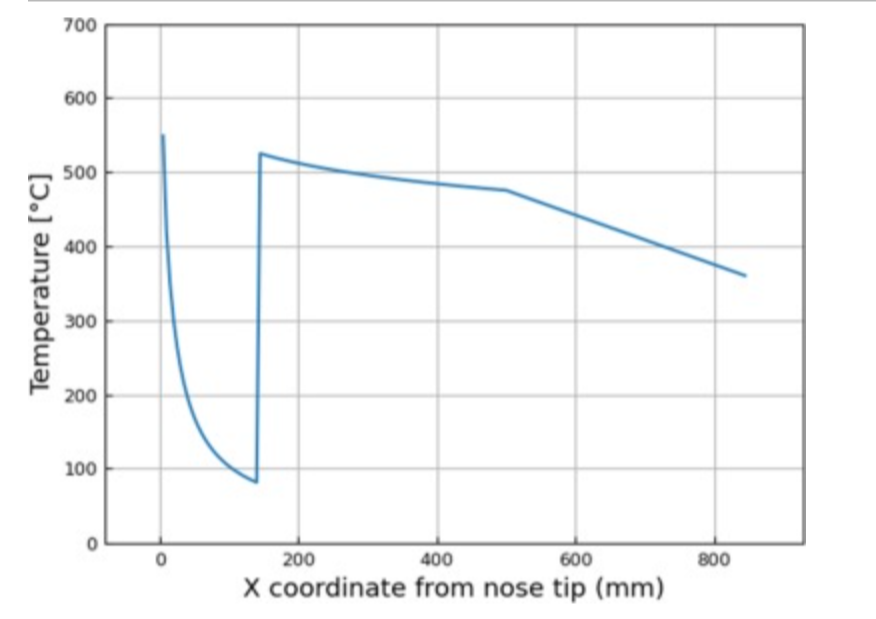
\includegraphics[width=0.6\textwidth]{images/temp-vs-x}
    \caption{Temperature as a function of distance down the vehicle. From Into the Black II (\cite{into-black}).}
    \label{figure:temp-vs-x}
\end{figure}
